\subsection{\large{Разработка расчётной модели данных}}
\addcontentsline{toc}{subsection}

Расчётная модель данных состоит из расчётных элементов. Ниже представлена общая диаграмма классов расчётной модели данных
(см. рис.\ref{pic:implementation__model-classes}).

\begin{figure}[H]
	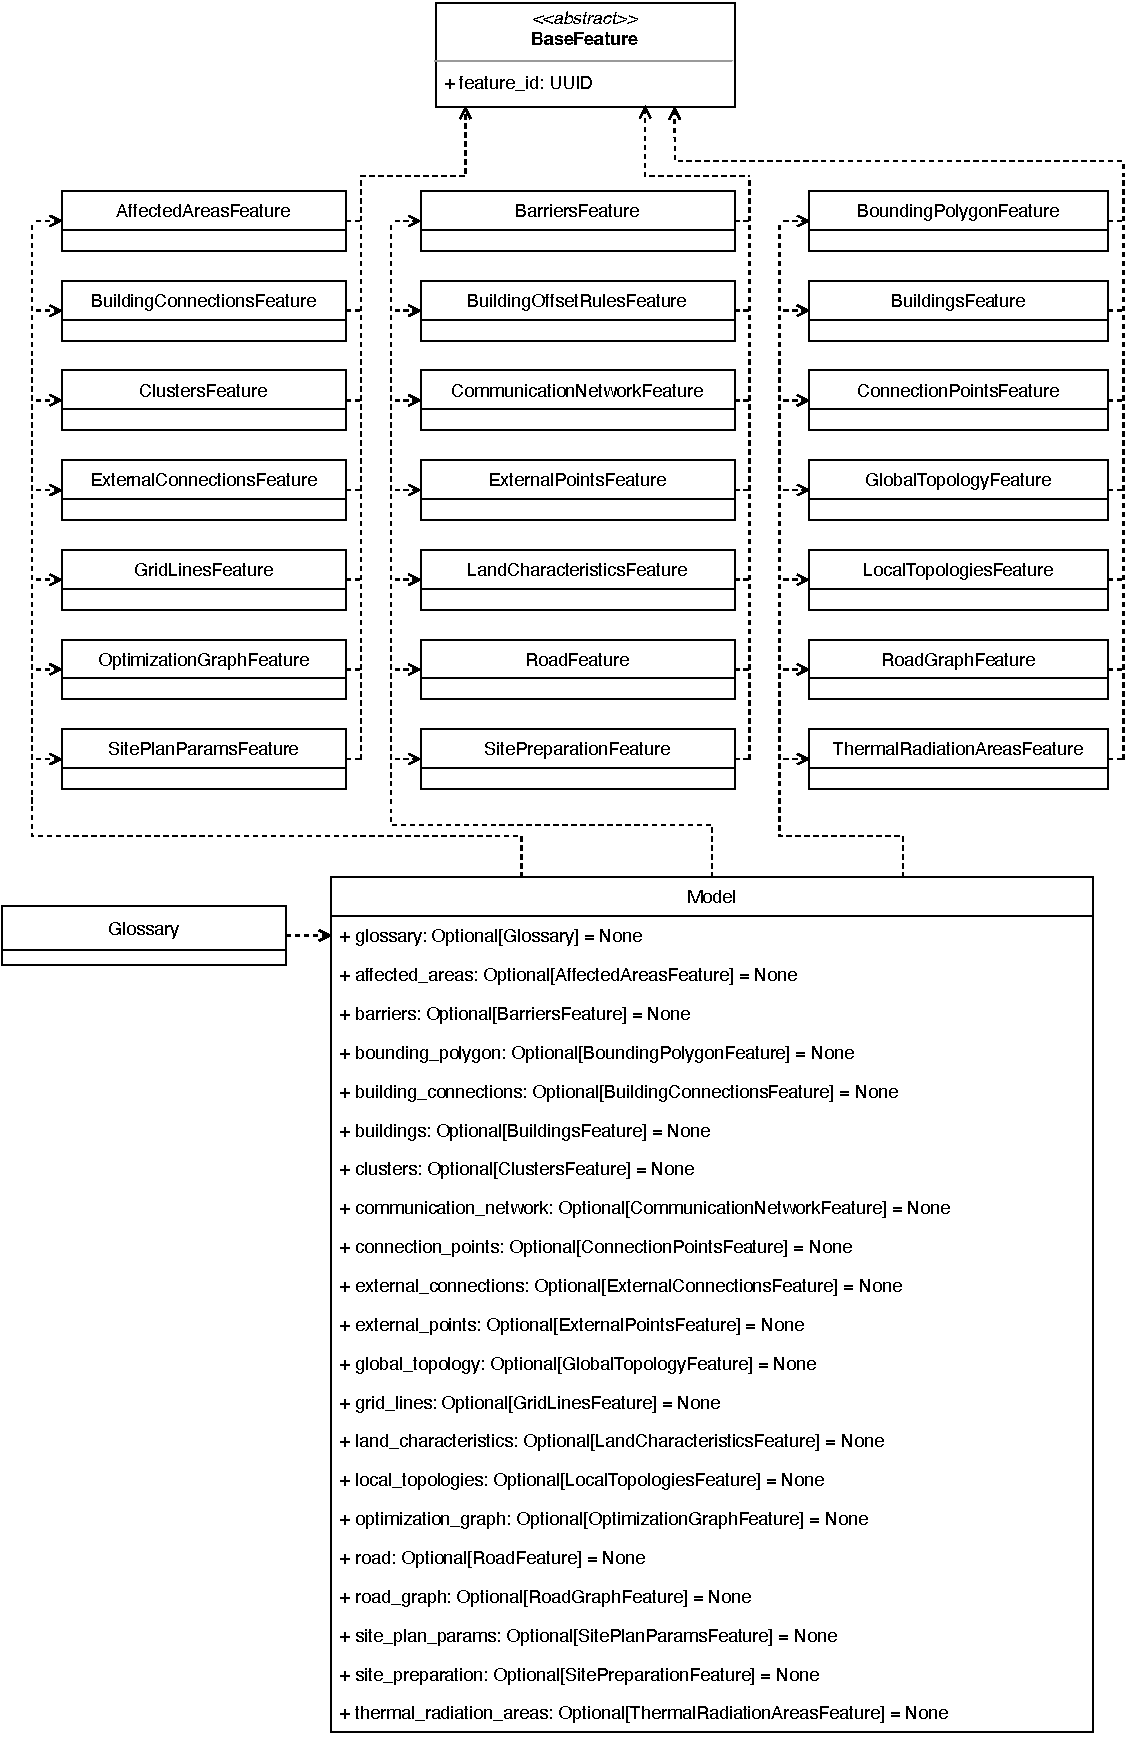
\includegraphics[width=0.8\textwidth]{implementation/pictures/model/classes}
	\caption{Общая диаграммма классов расчётной модели}
	\label{pic:implementation__model-classes}
\end{figure}
\vskip 5 mm

А вот диаграмма классов для расчётного элемента, описывающее сооружения(см. рис.\ref{pic:implementation__model-feature}).
\begin{figure}[H]
	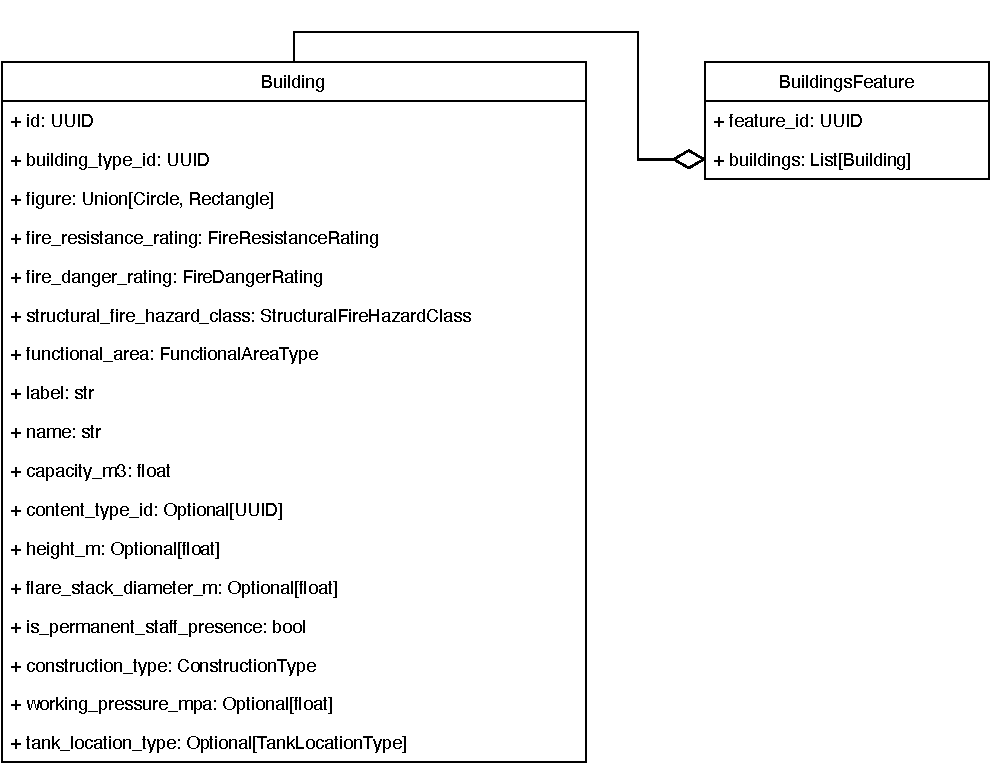
\includegraphics[width=0.8\textwidth]{implementation/pictures/model/feature}
	\caption{Общая диаграммма классов расчётной модели}
	\label{pic:implementation__model-feature}
\end{figure}

